\section{Background shape parametrization}
\label{sec:background}

%In our analysis, we employ two different background estimation techniques:
%\begin{itemize}
%\item {\bf analytic parameterization}: a smoothly falling function, whose
%  parameters are constrained to data simultaneously with the search for
%  the signal peak.  As vastly simpler, this method is used across the
%  board.

%\item {\bf H-tagging mistag rate:} we also explored a method for based
%  on measuring the $\Hbb$ mistag rate in the control region, and then
%  applying it to the V+jet pretag sample.  This method has two advantages
%  over the previous one: it is slightly better (the average limit for
%  $\Hbb$ channel is better by about 50~\GeVcc).  And, much more importantly,
%  it is obtained from a statistically independent sample, and comes with
%  both the full shape and normalization; as such, it is more suitable for
%  discovery.  This method, however, has one significant disadvantage -- it
%  is very labor intensive; this is especially important in a measurement
%%  such as this one where there are many channels.  We therefore use this
%  method as a cross-check, and present it's results in the appendix.

%\end{itemize}

Background from multijet events is modelled by a smoothly falling
distribution for each event category, given by the empirical
probability density function
\begin{equation}
P_D(m_\mathrm{jj}) = \frac{P_{0} (1 - m_\mathrm{jj}/\sqrt{s})^{P_{1}}}{(m_\mathrm{jj}/\sqrt{s})^{P_{2}}} \ .
\label{eqParam}
\end{equation}
\noindent For each category, the normalization factor $P_0$ and the
two parameters $P_1$ and $P_2$ are treated as uncorrelated. This
parameterization was deployed successfully in searches in dijet mass
spectra~\cite{cmsdijet}. A Fisher F-test~\cite{Ftest} is used to check
that no additional parameters are needed to model the individual
background distribution, for each of the four cases considered.

The background-only fit plot is only to demonstrate
 that the fit function works nice if no signal is assumed.
 However we don't use that function.
We search for a peak on top of the falling background spectrum by
means of a maximum likelihood fit to the data.

Figure \ref{fig:HbbZqqBG} and Figure \ref{fig:HwwZqqBG} show the dijet
 mass spectra from
H(bb)V-tagged and H(ww)V-tagged data 
fitted to Eq.~(\ref{eqParam}), respectively. 
The bottom panes show corresponding pull
distributions, demonstrating the agreement between the background-only
probability density function and the data.

The largest resonance mass in each channel is described 
in Table~\ref{table:highestMass}

\begin{table}[htbp]
\begin{center}
\caption{Highest resonance mass in each channel.}
\label{table:highestMass}
\begin{tabular}{cc}
\hline
%Channel & \multicolumn{1}{l|}{Resoanance(GeV)} \\ \hline
Category & Resonance(GeV) \\ \hline
%HbbVqq H-tag, high-purity V-tag& 2481 \\ 
Hbb1 & 2481 \\ 
%HbbVqq H-tag, low-purity V-tag & 2354 \\ 
Hbb2 & 2354 \\ 
%HwwVqq high-purity V\&V-tag& 2449 \\
Hww1 & 2449 \\
%HwwVqq low-purity H-tag, high-purity V-tag & 2448 \\ 
Hww2 & 2448 \\ 
%HwwVqq low-purity V-tag, high-purity H-tag & 2471 \\ \hline
Hww3 & 2471 \\ \hline
\end{tabular}
\end{center}
\end{table}



No sizeable deviation from the background-only hypothesis is seen,
exclusion limits are set on the product of cross section, 
acceptance, and branching fraction for
V' to HV search. 


%Figure \ref{fig:HwwZqqBG} shows the dijet mass spectra from
%HZ-tagged data fitted to Eq.~(\ref{eqParam}) and the bottom panes show corresponding pull
%distributions, demonstrating the agreement between the background-only
%probability density function and the data.

%No sizeable deviation from the background-only hypothesis is seen,
%exclusion limits are set on the product of cross section, acceptance, and branching fraction for
%Z' to H(ww)Z(qq) to all hadronic final states. 
%the five considered final states: qW, qZ, WW, WZ, and ZZ.


\begin{figure}[th!b]
\begin{center}
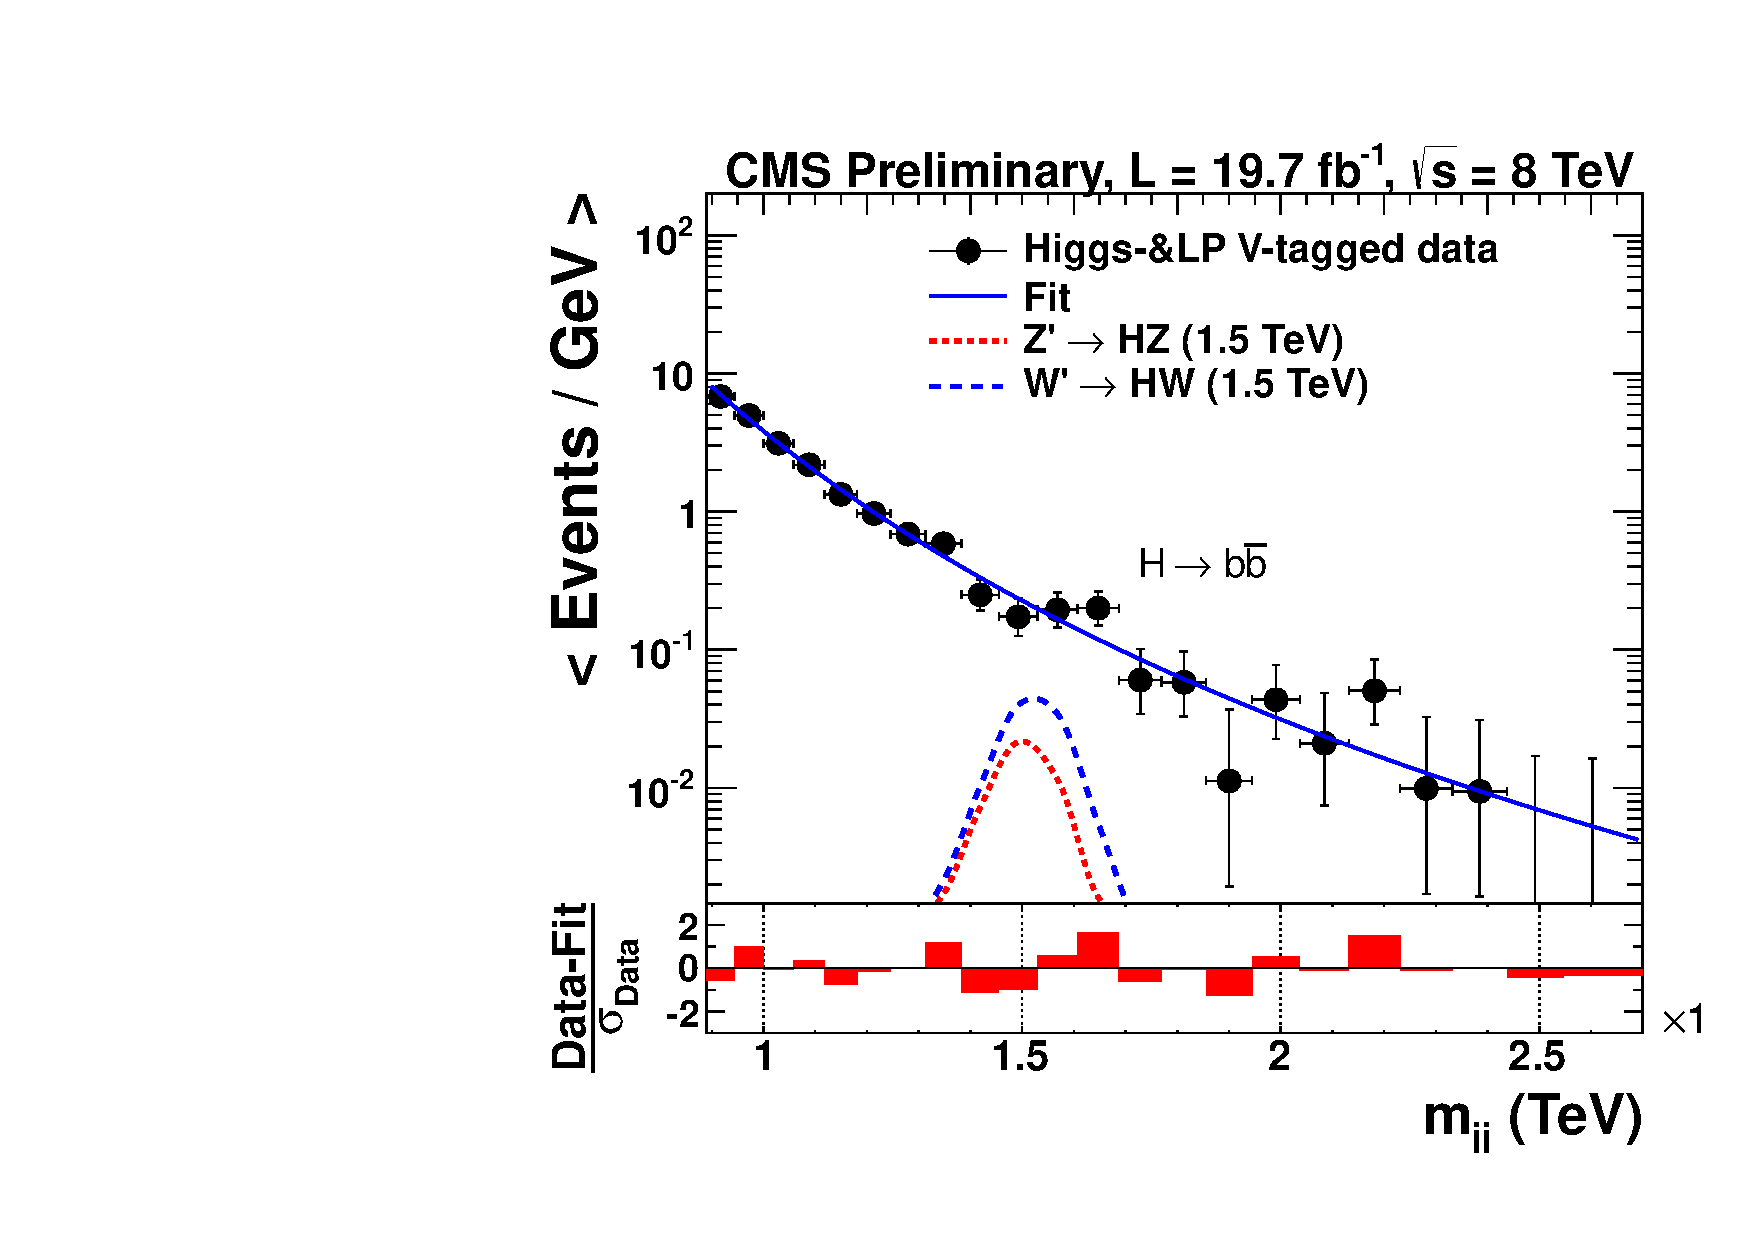
\includegraphics[width=0.49\textwidth]{EXO-14-009/HbbZqqfigs/FITS/HbbVqqFitAndPullLowP.pdf}
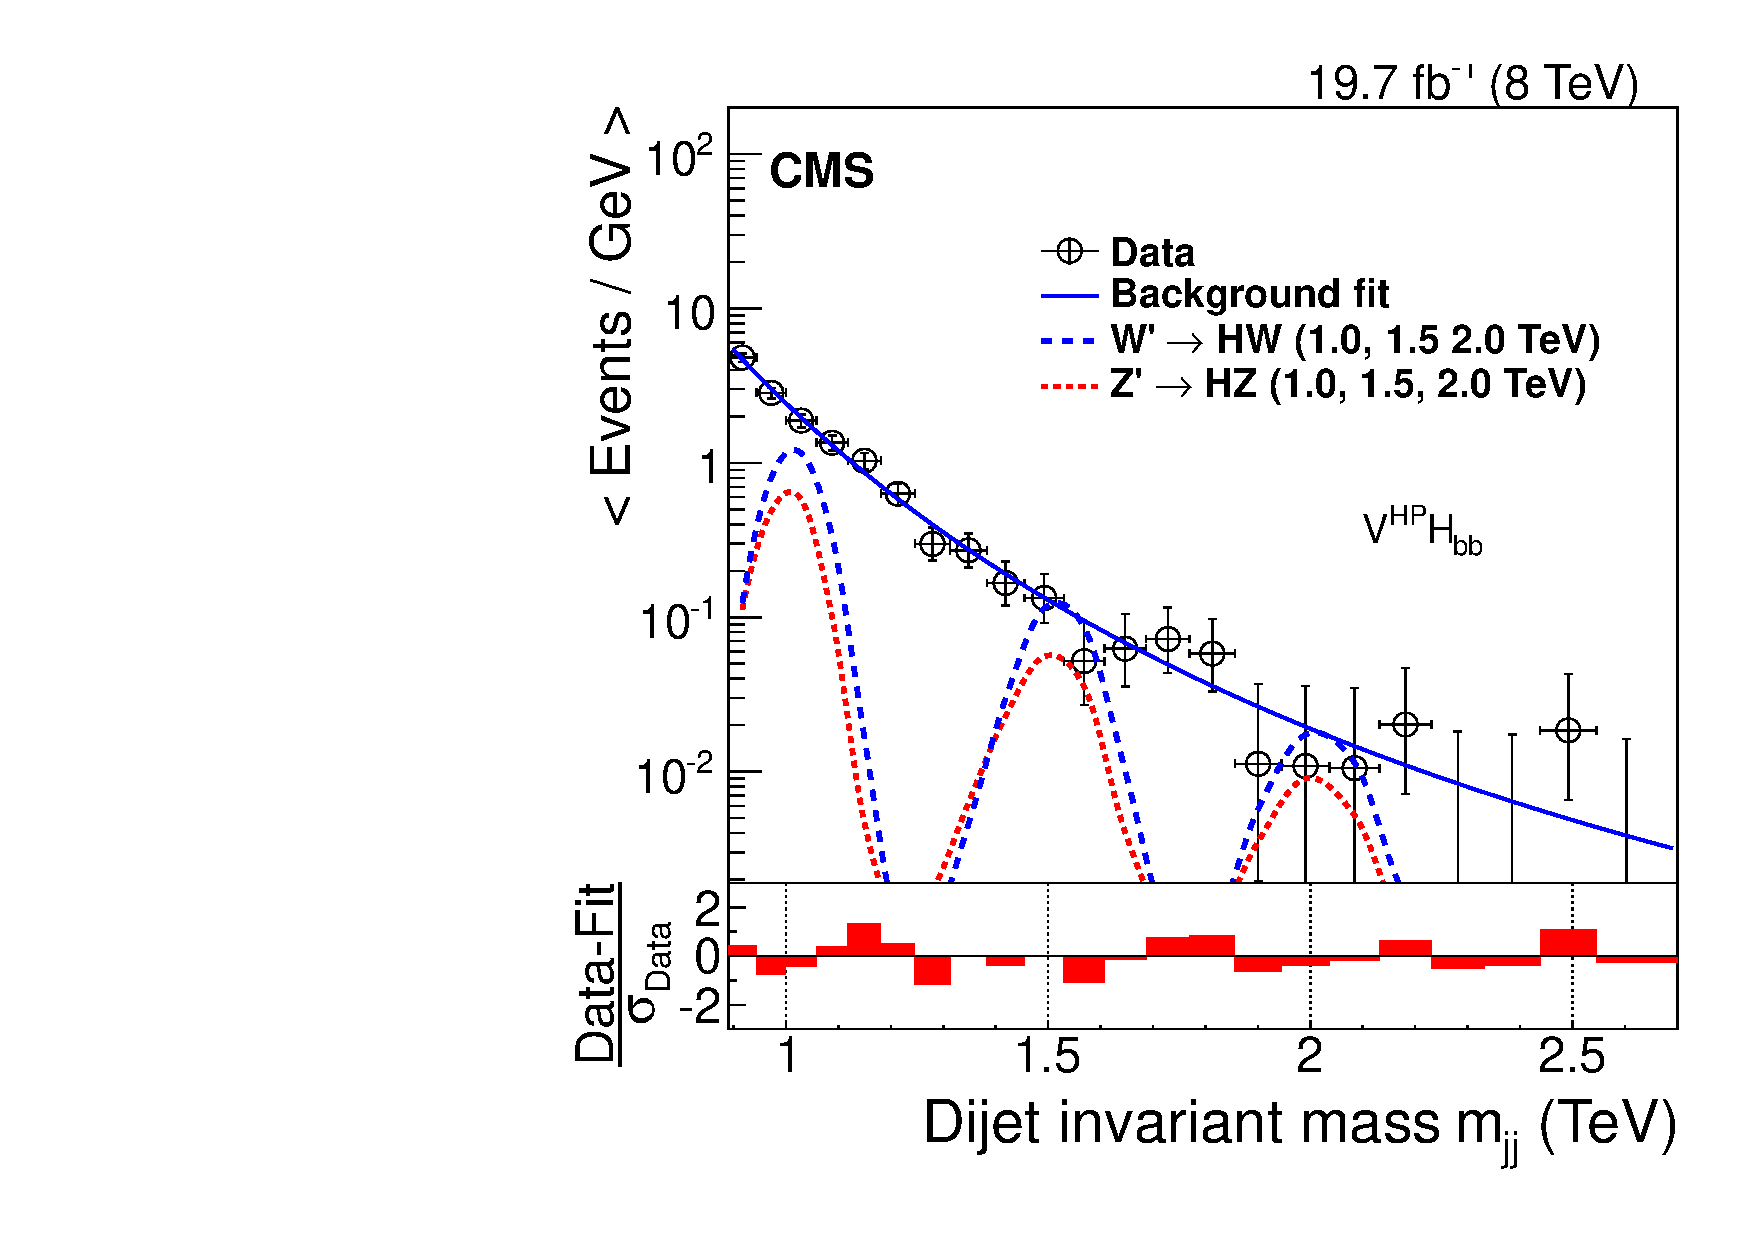
\includegraphics[width=0.49\textwidth]{EXO-14-009/HbbZqqfigs/FITS/HbbVqqFitAndPullHighP.pdf}
\end{center}
\caption{Distributions in $m_\mathrm{jj}$, respectively, for
   LP V-tag(left), HP V-tag(right).
    The solid curves represent the
   results of fitting Eq.~(\ref{eqParam}) to the data. The
   distributions for \HbbZqq\  and \HbbWqq\
   contributions, scaled to their corresponding cross sections, are
   given by the dash-dotted curves. Horizontal bars
in data indicates variable binning size. The corresponding pull
   distributions
   ($\frac{\text{Data}-\text{Fit}}{\sigma_{\text{Data}}}$, where
   $\sigma_{\text{Data}}$ represents the statistical uncertainty in
   the data in a bin in $m_\mathrm{jj}$) are shown below each
   $m_\mathrm{jj}$ plot.}
\label{fig:HbbZqqBG}
\end{figure}



\begin{figure}[th!b]
\begin{center}
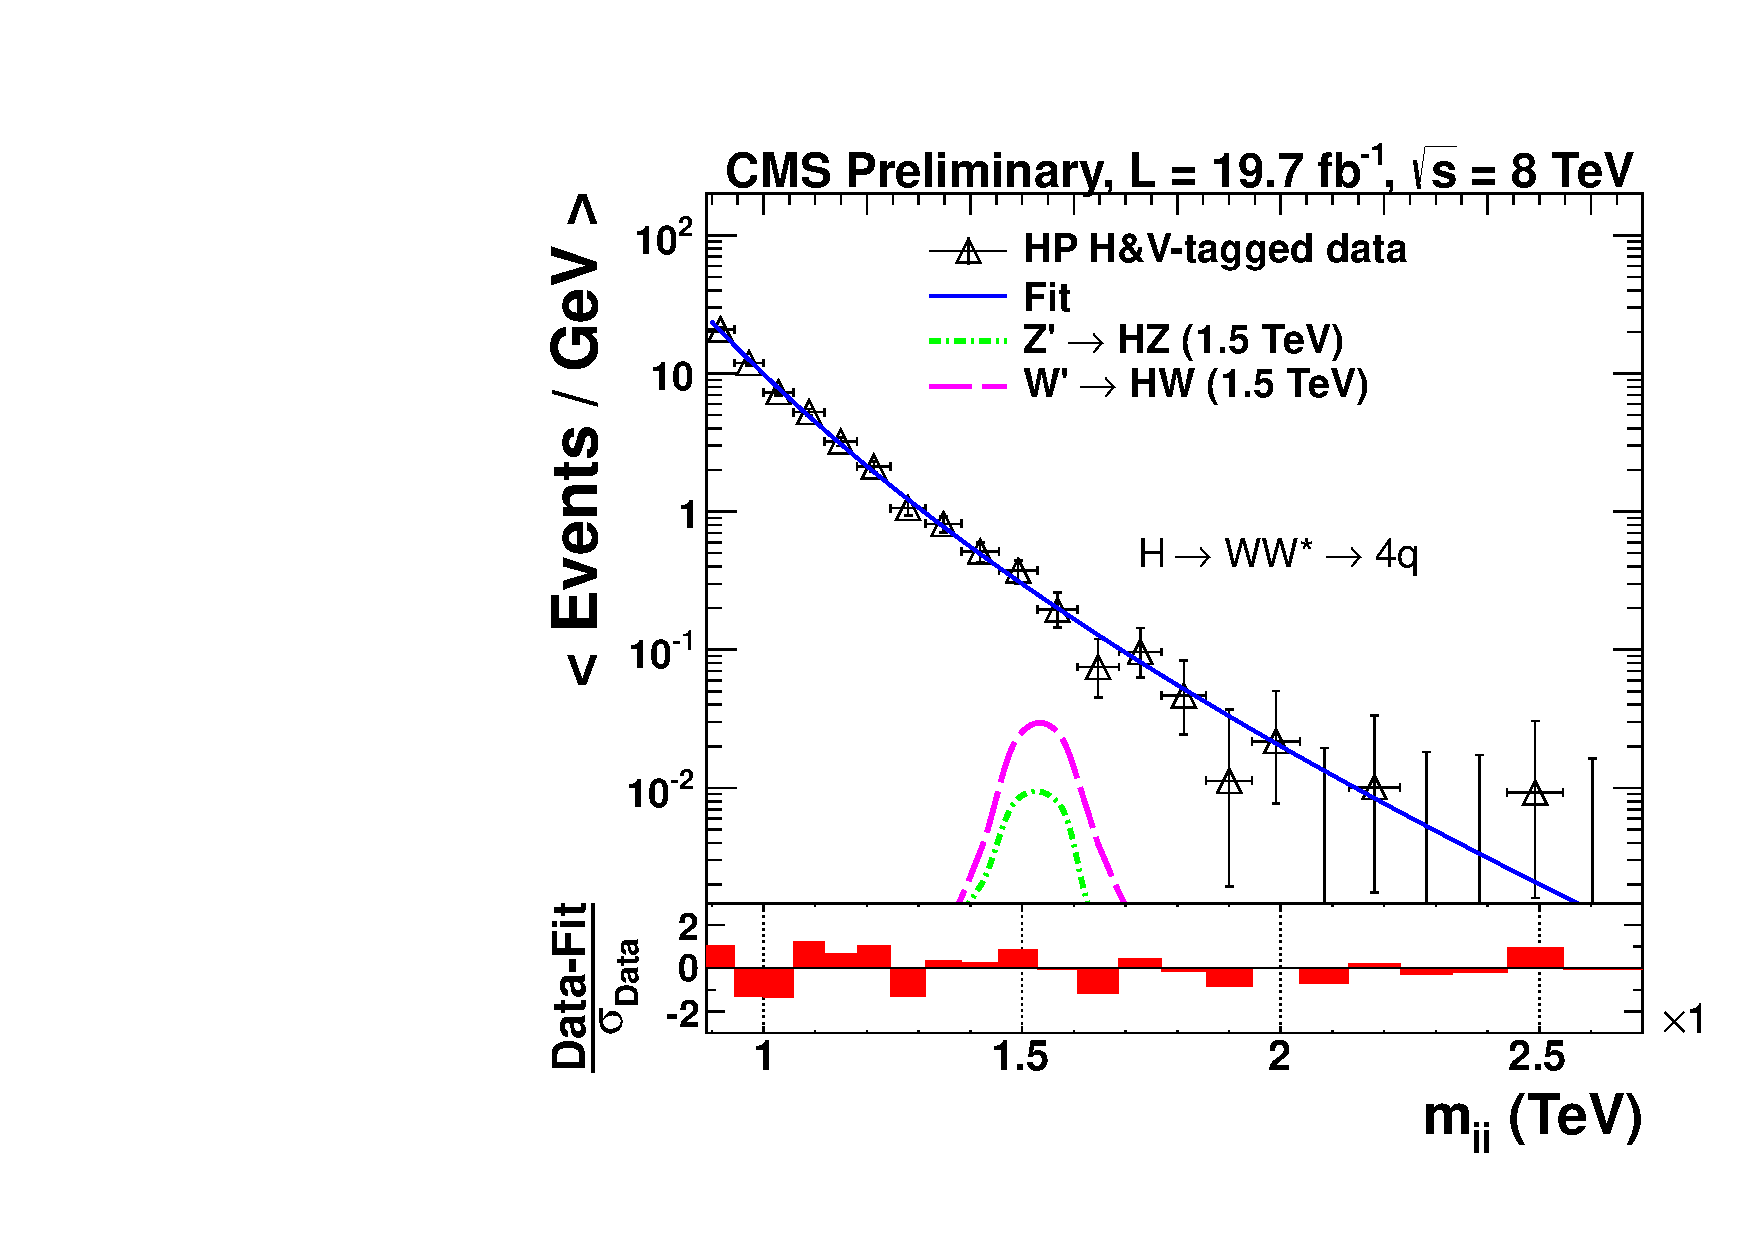
\includegraphics[width=0.69\textwidth]{EXO-14-009/HqqqqZqqfigs/FITS/HwwVqqFitAndPullHighP.pdf}
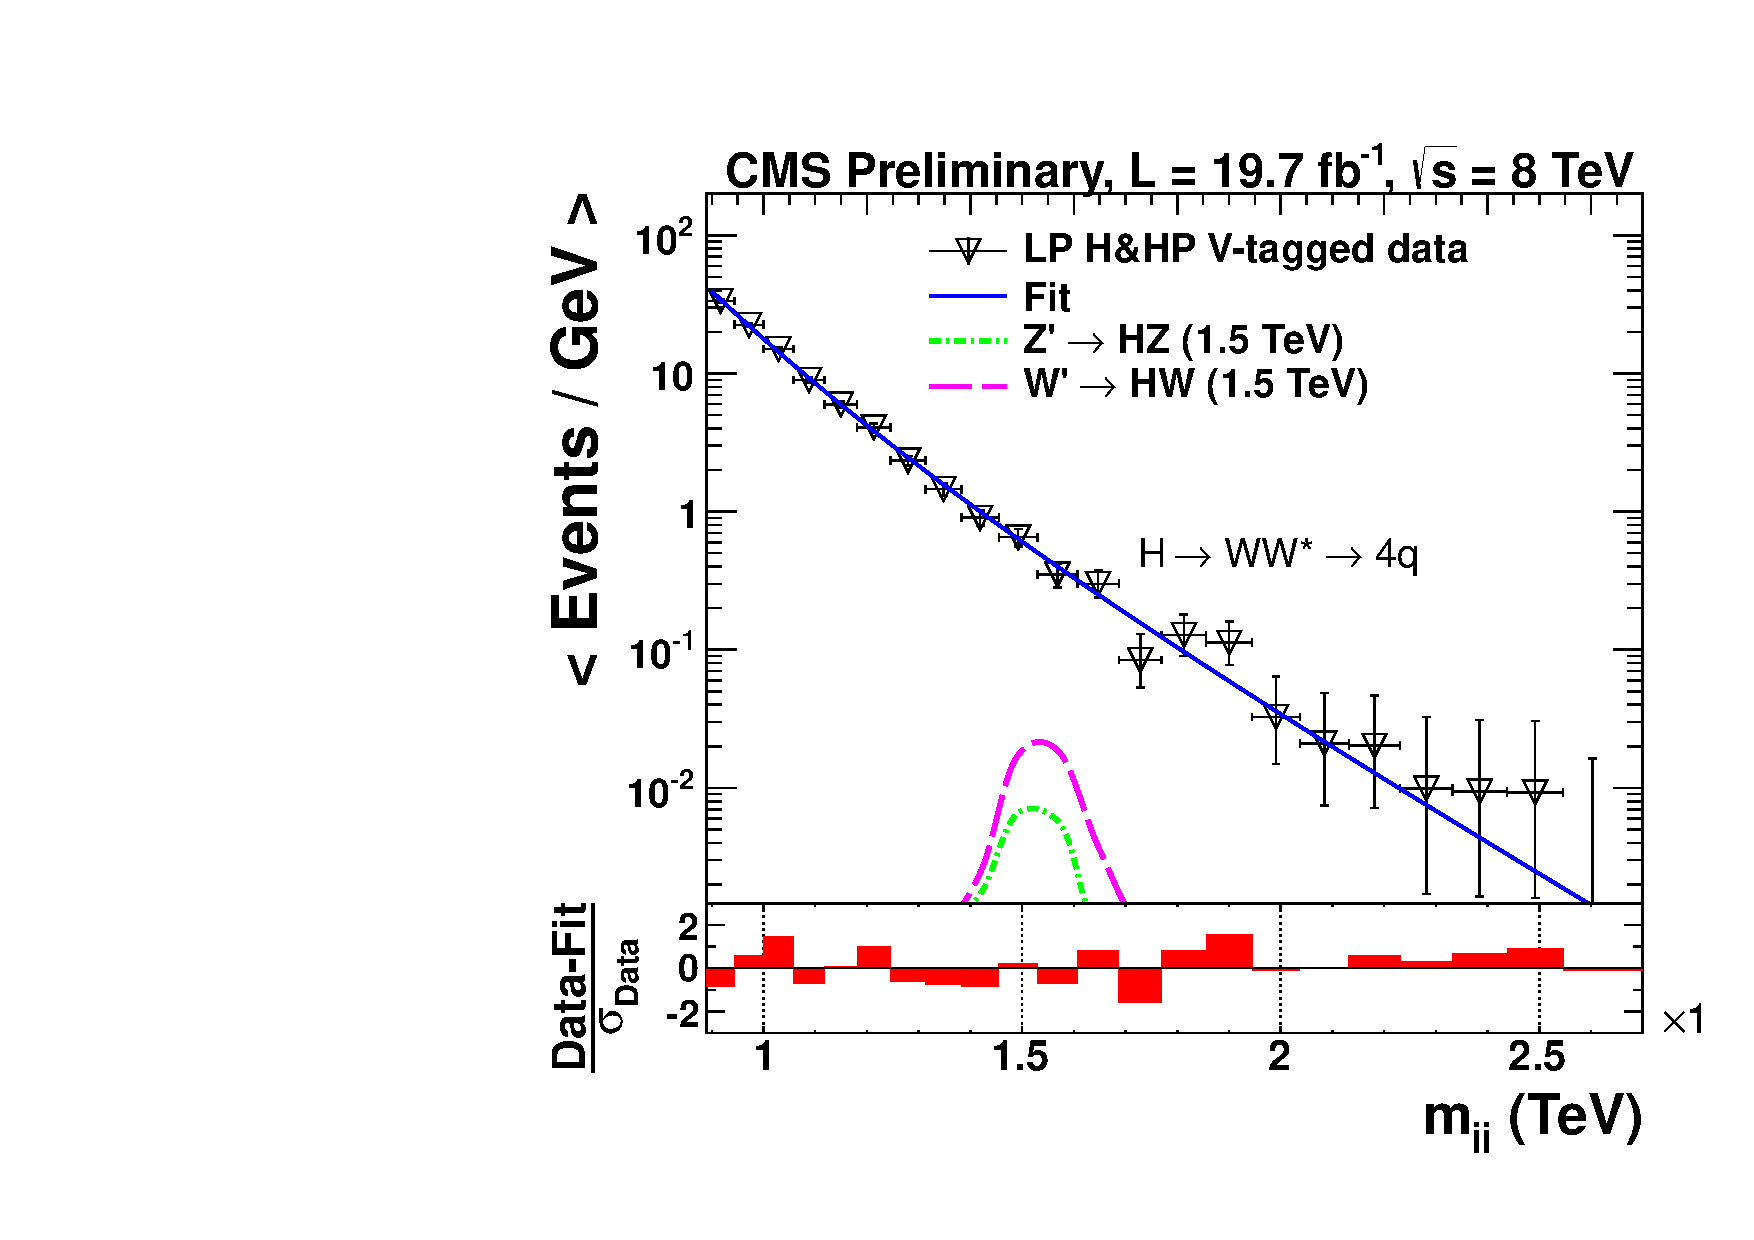
\includegraphics[width=0.49\textwidth]{EXO-14-009/HqqqqZqqfigs/FITS/HwwVqqFitAndPullLowH.pdf}
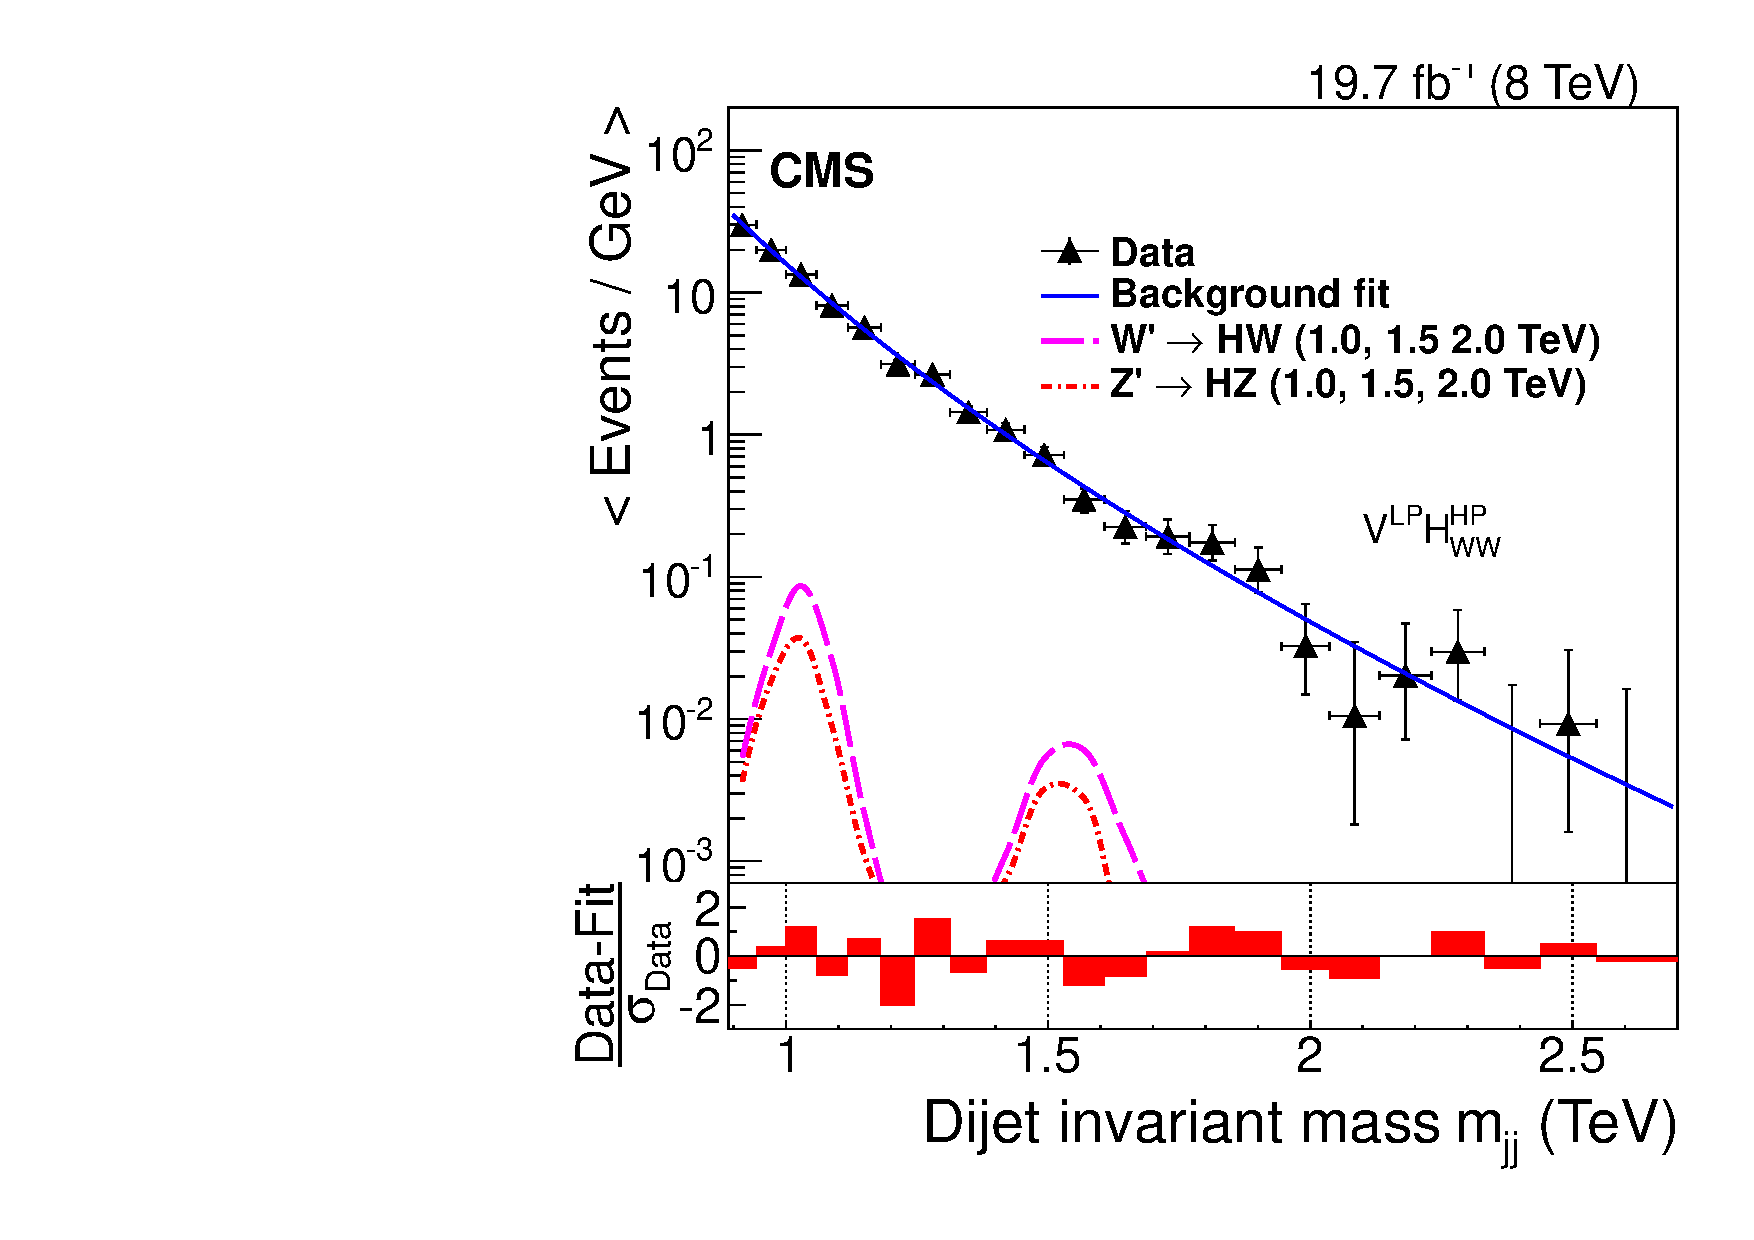
\includegraphics[width=0.49\textwidth]{EXO-14-009/HqqqqZqqfigs/FITS/HwwVqqFitAndPullLowV.pdf}
\end{center}
\caption{
Distributions in $m_\mathrm{jj}$, respectively, for
   HP(top), LP H-tag(bottom left) and
   LP V-tag(bottom right).
    The solid curves represent the
   results of fitting Eq.~(\ref{eqParam}) to the data. The
   distributions for \HwwWqq\ and \HwwZqq\
   contributions, scaled to their corresponding cross sections, are
   given by the dash-dotted curves. Horizontal bars
in data indicates variable binning size.
The corresponding pull
   distributions
   ($\frac{\text{Data}-\text{Fit}}{\sigma_{\text{Data}}}$, where
   $\sigma_{\text{Data}}$ represents the statistical uncertainty in
   the data in a bin in $m_\mathrm{jj}$) are shown below each
   $m_\mathrm{jj}$ plot. }
\label{fig:HwwZqqBG}
\end{figure}


\clearpage

